\chapter{Background}
\label{chap:background}

This chapter introduces the statistical background needed to study similarity between football players from a multivariate latent-space perspective. The main object of interest in this master's thesis is the \emph{player--season observation}, that is, the aggregated statistical profile of a given player over a given season. Each observation is therefore described by multiple performance variables simultaneously, and the central challenge is to understand how such multivariate profiles can be represented, compared, and interpreted in a lower-dimensional space.

More broadly, the aim is to construct statistical representations of player performance that make stylistic similarity empirically assessable. In this setting, similarity is not understood as a directly observed quantity, but as a latent relational structure induced by the joint behaviour of many football variables. This naturally places the problem within the scope of multivariate analysis, where the goal is often to reduce complexity while preserving the main patterns of variation, dependence, and association across observations.

The player--season construction also introduces a repeated-observation component, since some players appear in more than one season. This suggests that player profiles may exhibit persistence or variation over time. This feature of the data is kept in mind as a possible motivation for richer latent-variable formulations if the descriptive and probabilistic analyses indicate that such extensions are warranted. 

From a modelling perspective, the chapter develops the background in three parts. First, we review the general multivariate setting of the problem and the idea of representing high-dimensional football data in a smaller number of latent dimensions. Second, we discuss classical low-dimensional descriptive tools---in particular principal component analysis, factor analysis, and classical multidimensional scaling---which are useful for exploratory structure discovery and for identifying interpretable geometric or latent patterns in the data. Third, we introduce probabilistic counterparts to these descriptive ideas, with particular attention to Bayesian latent-space formulations that can incorporate uncertainty directly into the representation.

The need for this background is already visible in the exploratory analysis conducted on the player--season dataset. The data are built from event-based football statistics provided by \emph{Wyscout}, a professional football data platform that collects and structures detailed match event information for scouting and performance analysis. From these event records, season-level aggregates are constructed and organised into football-relevant blocks such as offensive production, progression and chance creation, carrying and one-versus-one actions, defensive activity, and duels. Once such multivariate profiles are defined, a number of statistical questions arise naturally: how many latent dimensions are needed to summarise the main structure, whether the variables reflect a smaller number of underlying stylistic components, and whether the resulting representation is stable and interpretable enough to support meaningful comparisons between players.

Beyond their descriptive value, these representations may also be relevant for downstream applications in recruitment and squad planning. A low-dimensional latent representation of player--season profiles can provide a structured way to compare footballers, identify stylistic neighbours, and understand how players relate to broader positional or tactical archetypes. In this thesis, several descriptive approaches---including principal component analysis, factor analysis, and multidimensional scaling---are explored as candidate tools for this purpose, after which greater emphasis is placed on probabilistic analogues that can represent latent structure while also quantifying uncertainty.

\section{Similarity representation}

In multivariate analysis, comparing observations requires some rule for translating several variables into a single notion of proximity. This can be done through methods that work directly with covariance or correlation structure, or through a similarity or dissimilarity measure defined on the observed feature vectors. In either case, the underlying issue is the same: different comparison rules emphasize different aspects of the data and may therefore induce different low-dimensional representations.

This point is especially relevant when observations are interpreted as performance profiles. Two player--season observations may be regarded as similar because they have similar magnitudes across variables, because they exhibit similar relative patterns across variables, or because they align along a common latent direction even if their absolute levels differ. Thus, similarity is not a uniquely defined property of the data, but rather a statistical construct that depends on how the multivariate profile is represented and compared.

In the present work, the player--season observations are built from weighted football features summarising different aspects of performance. After suitable preprocessing, standardisation, and block-wise weighting, two comparison rules are considered as initial descriptive choices. The first is the Euclidean distance between observations $x_i,x_j \in \mathbb{R}^p$,

\[
d_E(x_i,x_j)=\left(\sum_{k=1}^p (x_{ik}-x_{jk})^2\right)^{1/2}.
\]

This measure is sensitive to overall discrepancies in the feature space and therefore reflects differences in absolute profile location after the chosen transformations have been applied.

The second is a cosine-based dissimilarity, defined as

\[
d_C(x_i,x_j)=1-\frac{x_i^\top x_j}{\|x_i\|\,\|x_j\|}.
\]

This quantity depends on the angle between the two feature vectors and therefore emphasises profile orientation relative to the origin rather than absolute separation in feature space. Strictly speaking, \(d_C\) is not a metric distance: \(d_C(x_i,x_j)=0\) implies that \(x_i\) and \(x_j\) have the same direction, but not necessarily that \(x_i=x_j\).

This distinction is important because this cosine dissimilarity and Pearson correlation use different reference points. Cosine dissimilarity compares vectors relative to the origin, whereas correlation compares centred profiles. In particular, if \(\tilde{x}_i=x_i-\bar{x}_i\) and \(\tilde{x}_j=x_j-\bar{x}_j\), then
\[
\operatorname{corr}(x_i,x_j)
=
\frac{\tilde{x}_i^\top \tilde{x}_j}
{\|\tilde{x}_i\|\,\|\tilde{x}_j\|}.
\]
Thus, correlation is the cosine dissimilarity between centred profiles. This makes correlation relevant for the later PCA and factor-analytic modelling, since these methods are directly based on covariance/correlation structure.

These two measures are not intended to exhaust the set of reasonable comparisons in multivariate statistics. Rather, they provide two conceptually distinct and practically useful benchmarks for the exploratory stage of the analysis: one based more directly on geometric separation in the transformed feature space, and one based on angular separation between multivariate profiles. Their comparison is informative precisely because the resulting similarity structures need not coincide.

\begin{figure}[h]
    \centering
    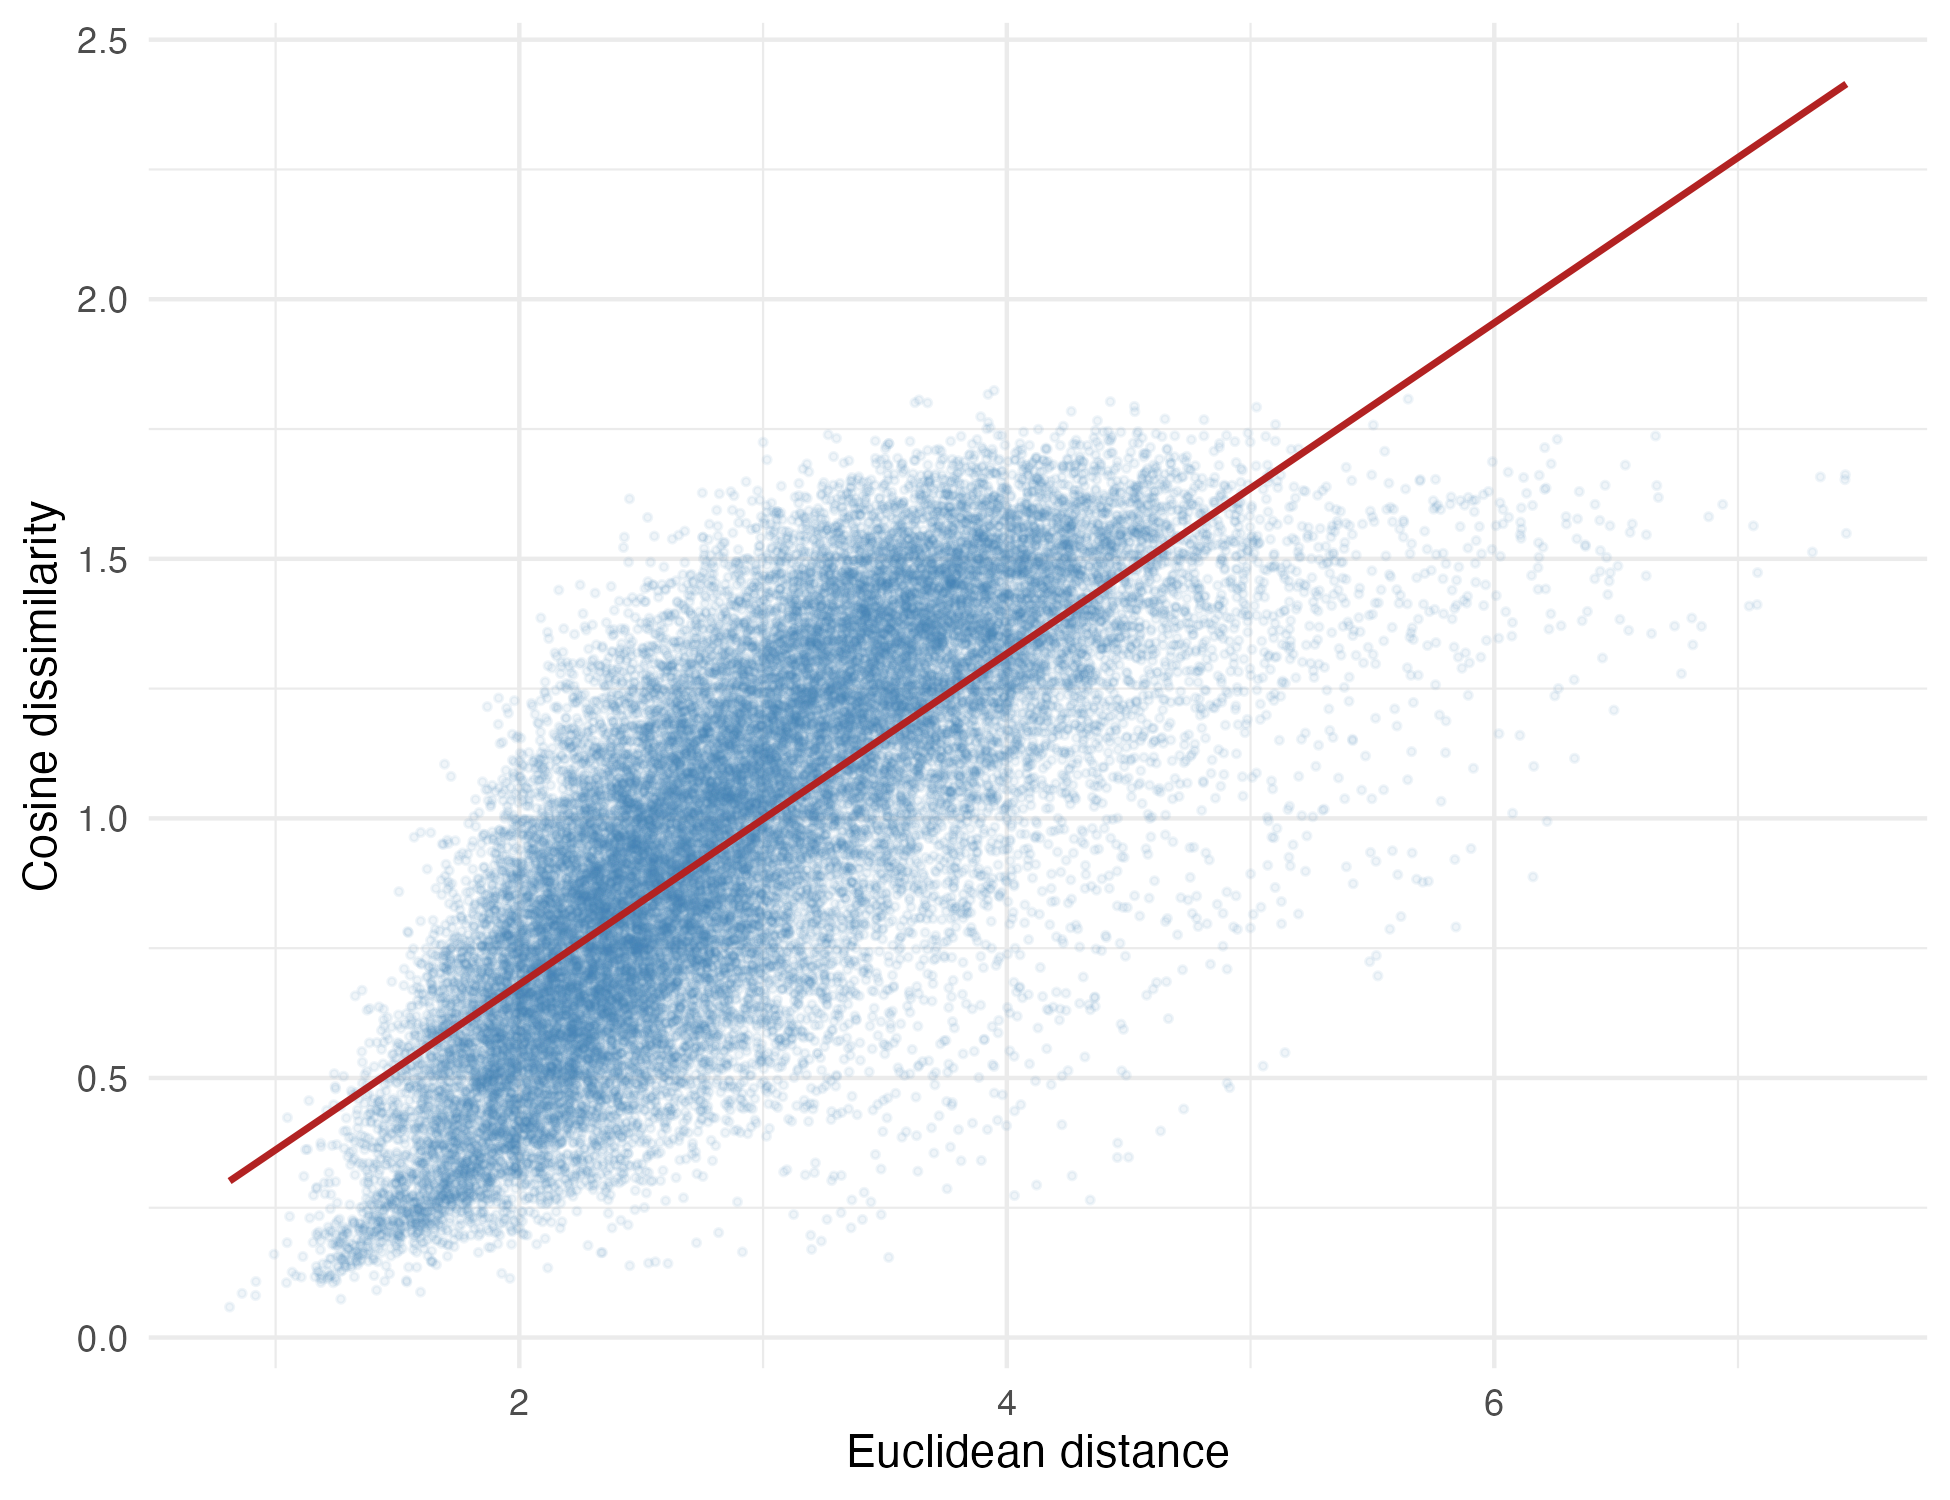
\includegraphics[width=0.8\textwidth]{images/scatter_distances.png}
    \caption{Pairwise Euclidean vs. cosine dissimilarities for the player-season subset (N = 900, ~30,000 sampled pairs). The two metrics show moderate-to-strong agreement (Pearson = 0.746, Spearman = 0.774).}
    \label{fig:scatter_dist}
\end{figure}

The exploratory results in \autoref{fig:scatter_dist} show that Euclidean distance and cosine dissimilarity are substantially related, but not equivalent. This is expected because both are computed from the same transformed feature vectors, while emphasising different aspects of them. Euclidean distance reflects absolute separation in the weighted standardised feature space, whereas cosine dissimilarity reflects angular separation relative to the origin. Consequently, the induced neighbourhood structure and the interpretation of player similarity may change depending on the comparison rule.

\section{Exploratory low-dimensional structure}

A natural question in multivariate analysis is whether a high-dimensional set of observations can be represented satisfactorily in a smaller number of dimensions without losing its main structural patterns. In the present work, this question is approached first through classical exploratory techniques, namely principal component analysis (PCA), factor analysis (FA), and classical multidimensional scaling (CMDS) \cite{jolliffe2002pca,bartholomew2011latent,borg2005mds}. These methods do not provide the final probabilistic framework of the work, but they are useful diagnostic tools for determining whether the feature space and the induced distance structure contain stable lower-dimensional patterns worth modelling.

Before specifying a richer latent-variable model, it is helpful to understand whether the data exhibits interpretable low-dimensional structure at all, whether such structure is approximately stable across relevant subsets of it, and whether the dominant structure is more naturally described through covariance/correlation patterns or through dissimilarities. In particular, exploratory analyses can be stratified or inspected by season, playing time, or positional group in order to assess whether a single global representation is plausible or whether the data suggest more heterogeneous structure that should later guide the modelling strategy.

These methods serve different but complementary purposes. PCA works directly on the feature matrix and identifies orthogonal linear combinations that explain as much sample variation as possible \cite{jolliffe2002pca}. FA also works on the feature matrix, but seeks a lower-rank latent structure capable of reproducing the dependence among the observed variables up to variable-specific residual variation \cite{bartholomew2011latent}. CMDS, by contrast, starts from a matrix of pairwise dissimilarities and searches for an embedding whose interpoint distances approximate the observed dissimilarities \cite{borg2005mds}. Taken together, these methods help address several preliminary questions: whether dimension reduction is plausible, whether the dominant axes or factors admit football interpretation, whether the conclusions are robust across relevant subsets of the data, and whether the structure suggested by the features is compatible with the structure suggested by the dissimilarities.

\subsection{Principal component analysis}

Let $\mathbf{X}=(x_{ij})\in\mathbb{R}^{n\times p}$ denote the feature matrix, where $n$ is the number of player--season observations and $p$ is the number of transformed and standardised football features retained for the analysis. In the present application, $n=4586$, corresponding to player--season rows, and the columns of $\mathbf{X}$ represent season-level statistics derived from Wyscout event data, including variables related to shooting, finishing, progression, passing, dribbling, defensive actions, recoveries, duels, and aerial involvement.

Principal component analysis (PCA) is a classical dimension-reduction technique that seeks linear combinations of the observed variables with maximal sample variance under orthogonality constraints \cite{jolliffe2002pca}. It is useful here as an exploratory device because it reveals whether the player--season feature space is dominated by a small number of broad directions of variation, and because it helps identify which football variables contribute most strongly to those directions.

To define PCA formally, let $\mathbf{x}_1,\ldots,\mathbf{x}_n\in\mathbb{R}^p$ denote the rows of $\mathbf{X}$, and assume that the columns of $\mathbf{X}$ have been centred. For any vector $\mathbf{v}\in\mathbb{R}^p$, define the projected sample scores
\[
z_i(\mathbf{v})=\mathbf{x}_i^\top \mathbf{v}, \qquad i=1,\ldots,n,
\]
and their sample variance
\[
\widehat{\mathrm{Var}}\bigl(z(\mathbf{v})\bigr)
=
\frac{1}{n-1}\sum_{i=1}^n \bigl(z_i(\mathbf{v})-\bar z(\mathbf{v})\bigr)^2.
\]

\begin{definition}
The first principal component direction is defined as
\[
\mathbf{v}_1
=
\arg\max_{\|\mathbf{v}\|=1}\widehat{\mathrm{Var}}\bigl(z(\mathbf{v})\bigr),
\]
and, recursively, for $k\geq 2$, the $k$-th principal component direction is defined as
\[
\mathbf{v}_k
=
\arg\max_{\substack{\|\mathbf{v}\|=1\\ \mathbf{v}\perp \mathbf{v}_1,\ldots,\mathbf{v}_{k-1}}}
\widehat{\mathrm{Var}}\bigl(z(\mathbf{v})\bigr).
\]
The vectors $\mathbf{v}_1,\ldots,\mathbf{v}_p$ are called the principal component directions, and the projected variables $\mathbf{X}\mathbf{v}_1,\ldots,\mathbf{X}\mathbf{v}_p$ are called the principal component scores.
\end{definition}

A standard result states that these directions are the eigenvectors of the sample covariance matrix of the centred data \cite{jolliffe2002pca}. If
\[
\mathbf{S}=\frac{1}{n-1}\mathbf{X}^\top\mathbf{X},
\]
then the principal component directions are given by the eigenvectors of $\mathbf{S}$, ordered by decreasing eigenvalue. The corresponding eigenvalues $\lambda_1\geq \cdots \geq \lambda_p$ are the sample variances explained by the successive components. If the analysis is instead performed on standardised variables, then one may equivalently work with the sample correlation matrix
\[
\mathbf{\Omega}
=
\frac{1}{n-1}\mathbf{Z}^\top\mathbf{Z},
\qquad
\mathbf{Z}
=
\left[
\frac{\mathbf{X}_{\cdot 1}-\bar X_1\mathbf{1}}{s_1},
\ldots,
\frac{\mathbf{X}_{\cdot p}-\bar X_p\mathbf{1}}{s_p}
\right],
\]
where $\bar{X_j}$ is the sample mean and $s_j$ is the sample standard deviation of the $j$-th variable \cite{jolliffe2002pca}. The coefficients of each eigenvector are commonly referred to as \emph{loadings}, while the coordinates of the observations after projection onto the component directions are the \emph{scores}.

PCA is used as an exploratory instrument applied only to the transformed football-feature matrix. Season identifiers, competition identifiers, player identifiers, player names, minutes played, and matches are not treated as active PCA variables; they are retained as metadata for interpretation and diagnostic checks. First, PCA provides a rough sense of whether the player--season feature space is intrinsically high-dimensional or whether a moderate number of directions captures a substantial proportion of sample variation. Second, the leading loadings indicate which football actions most strongly define the dominant axes of variation. Third, the component scores can be inspected across metadata-defined subsets---for instance by season, competition, or minutes played---to assess whether the same low-dimensional structure is broadly visible across the sample.

\begin{figure}[h]
    \centering
    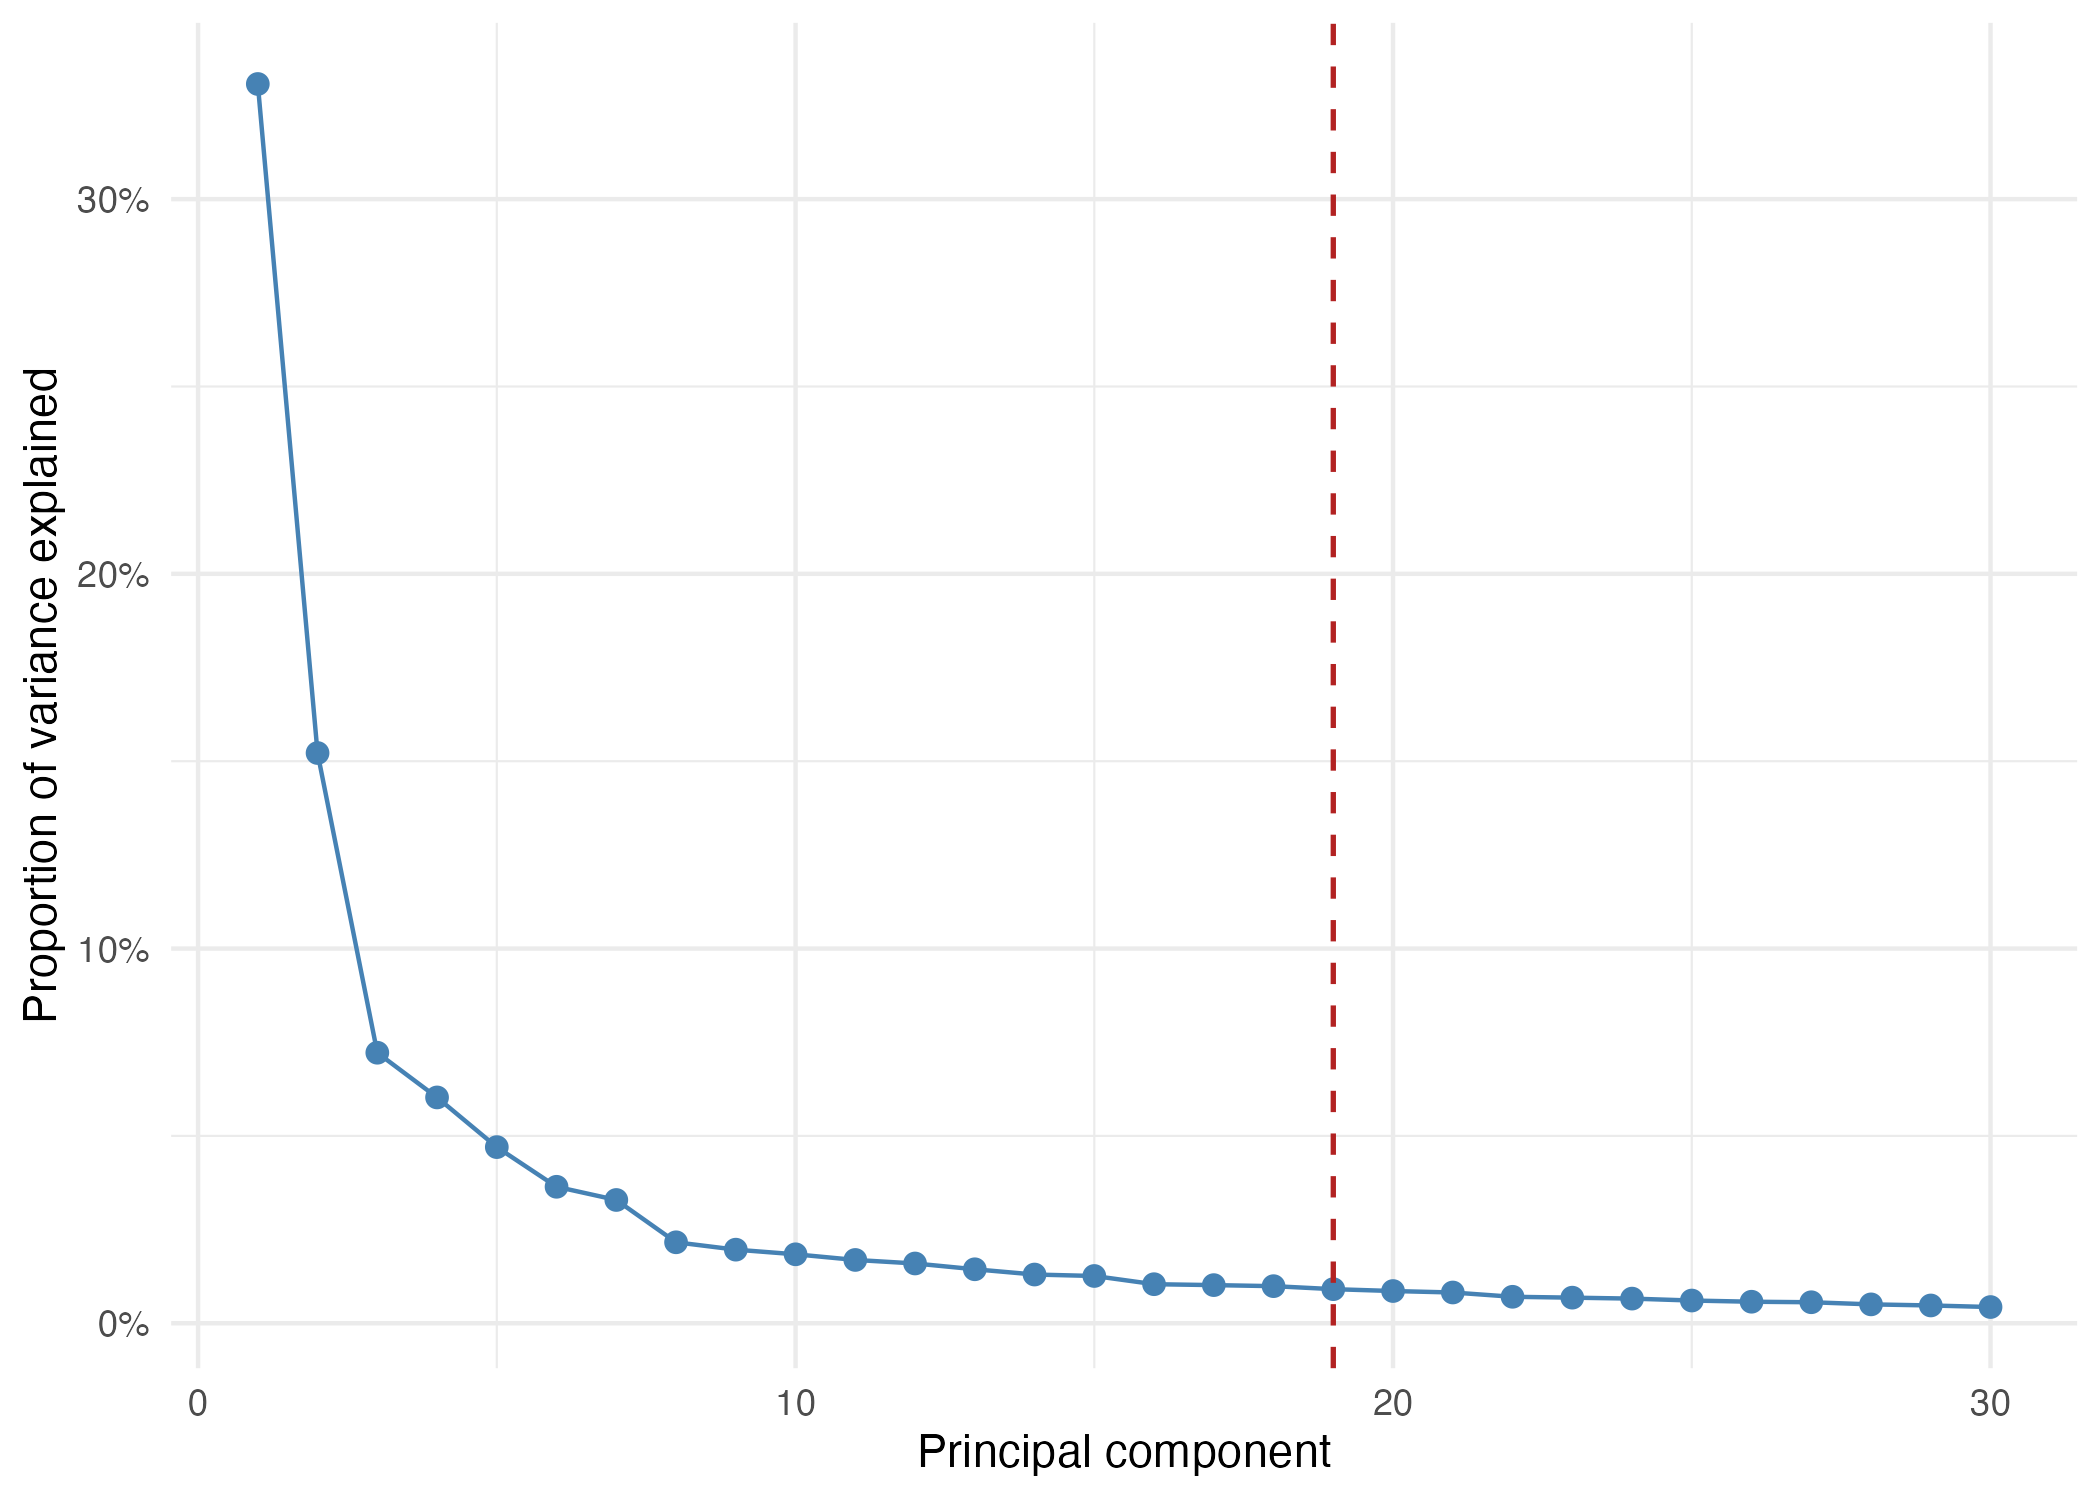
\includegraphics[width=0.8\textwidth]{images/scree_pca.png}
    \caption{Scree plot of the first 30 principal components. PC1 and PC2 jointly explain approximately \(48\%\) of the variance, while the first ten components explain approximately \(79\%\). The dashed line marks the first component count reaching at least \(90\%\) cumulative explained variance (nineteen components).}
    \label{fig:scree_plot}
\end{figure}

The exploratory results suggest that the data are structured but not trivially so. In particular, \autoref{fig:scree_plot} shows that the first two principal components explain \(48.3\%\) of the total sample variance, the first five around \(66.2\%\), and the first ten roughly \(79.1\%\). Using \(90\%\) cumulative explained variance as a descriptive threshold requires about nineteen principal components for a high-fidelity linear summary. This indicates that a low-dimensional summary is plausible, but also that the player--season feature space cannot be reduced to a single simple axis without substantial information loss: with \(P=48\) engineered features spanning finishing, passing, carrying, defending, and duelling, considerably more shared structure remains beyond the first few directions than a smaller, coarser feature set would suggest. To interpret the leading components beyond their explained variance, the variables with the largest absolute loadings were inspected. \autoref{tab:pca_loadings} reports the five largest absolute loadings for each of the first five principal components.

\begin{table}[h]
\centering
\caption{Largest absolute PCA loadings for the first five principal components.}
\label{tab:pca_loadings}
\begin{tabular}{llr}
\toprule
Component & Feature & Loading \\
\midrule
PC1 & \texttt{per90\_dribbles}          &  0.318 \\
PC1 & \texttt{per90\_touch\_in\_box}    &  0.251 \\
PC1 & \texttt{per90\_shots}             &  0.244 \\
PC1 & \texttt{per90\_accelerations}     &  0.229 \\
PC1 & \texttt{per90\_progressive\_run}  &  0.225 \\
\midrule
PC2 & \texttt{per90\_head\_shots}       & -0.298 \\
PC2 & \texttt{per90\_progressive\_run}  &  0.295 \\
PC2 & \texttt{per90\_accelerations}     &  0.279 \\
PC2 & \texttt{per90\_aerial\_duels}     & -0.242 \\
PC2 & \texttt{per90\_dribbles}          &  0.215 \\
\midrule
PC3 & \texttt{per90\_defensive\_duels}      & -0.342 \\
PC3 & \texttt{per90\_fouls}                 & -0.341 \\
PC3 & \texttt{rate\_successful\_dribbles}   &  0.303 \\
PC3 & \texttt{per90\_loose\_ball\_duels}    & -0.268 \\
PC3 & \texttt{per90\_dribbles\_against}     & -0.263 \\
\midrule
PC4 & \texttt{rate\_successful\_dribbles}       &  0.308 \\
PC4 & \texttt{per90\_accelerations}             & -0.299 \\
PC4 & \texttt{per90\_progressive\_run}          & -0.286 \\
PC4 & \texttt{per90\_passes\_to\_final\_third}  &  0.228 \\
PC4 & \texttt{per90\_through\_passes}           &  0.223 \\
\midrule
PC5 & \texttt{rate\_successful\_dribbles}   &  0.754 \\
PC5 & \texttt{rate\_offensive\_duels\_won}  &  0.281 \\
PC5 & \texttt{per90\_accelerations}         &  0.217 \\
PC5 & \texttt{per90\_progressive\_run}      &  0.177 \\
PC5 & \texttt{per90\_dribbles}              &  0.171 \\
\bottomrule
\end{tabular}
\end{table}

Interpretations based on the loadings are purely descriptive, and the signs of PCA loadings should not be over-interpreted because eigenvectors are identifiable only up to sign.

\begin{figure}[h]
    \centering
    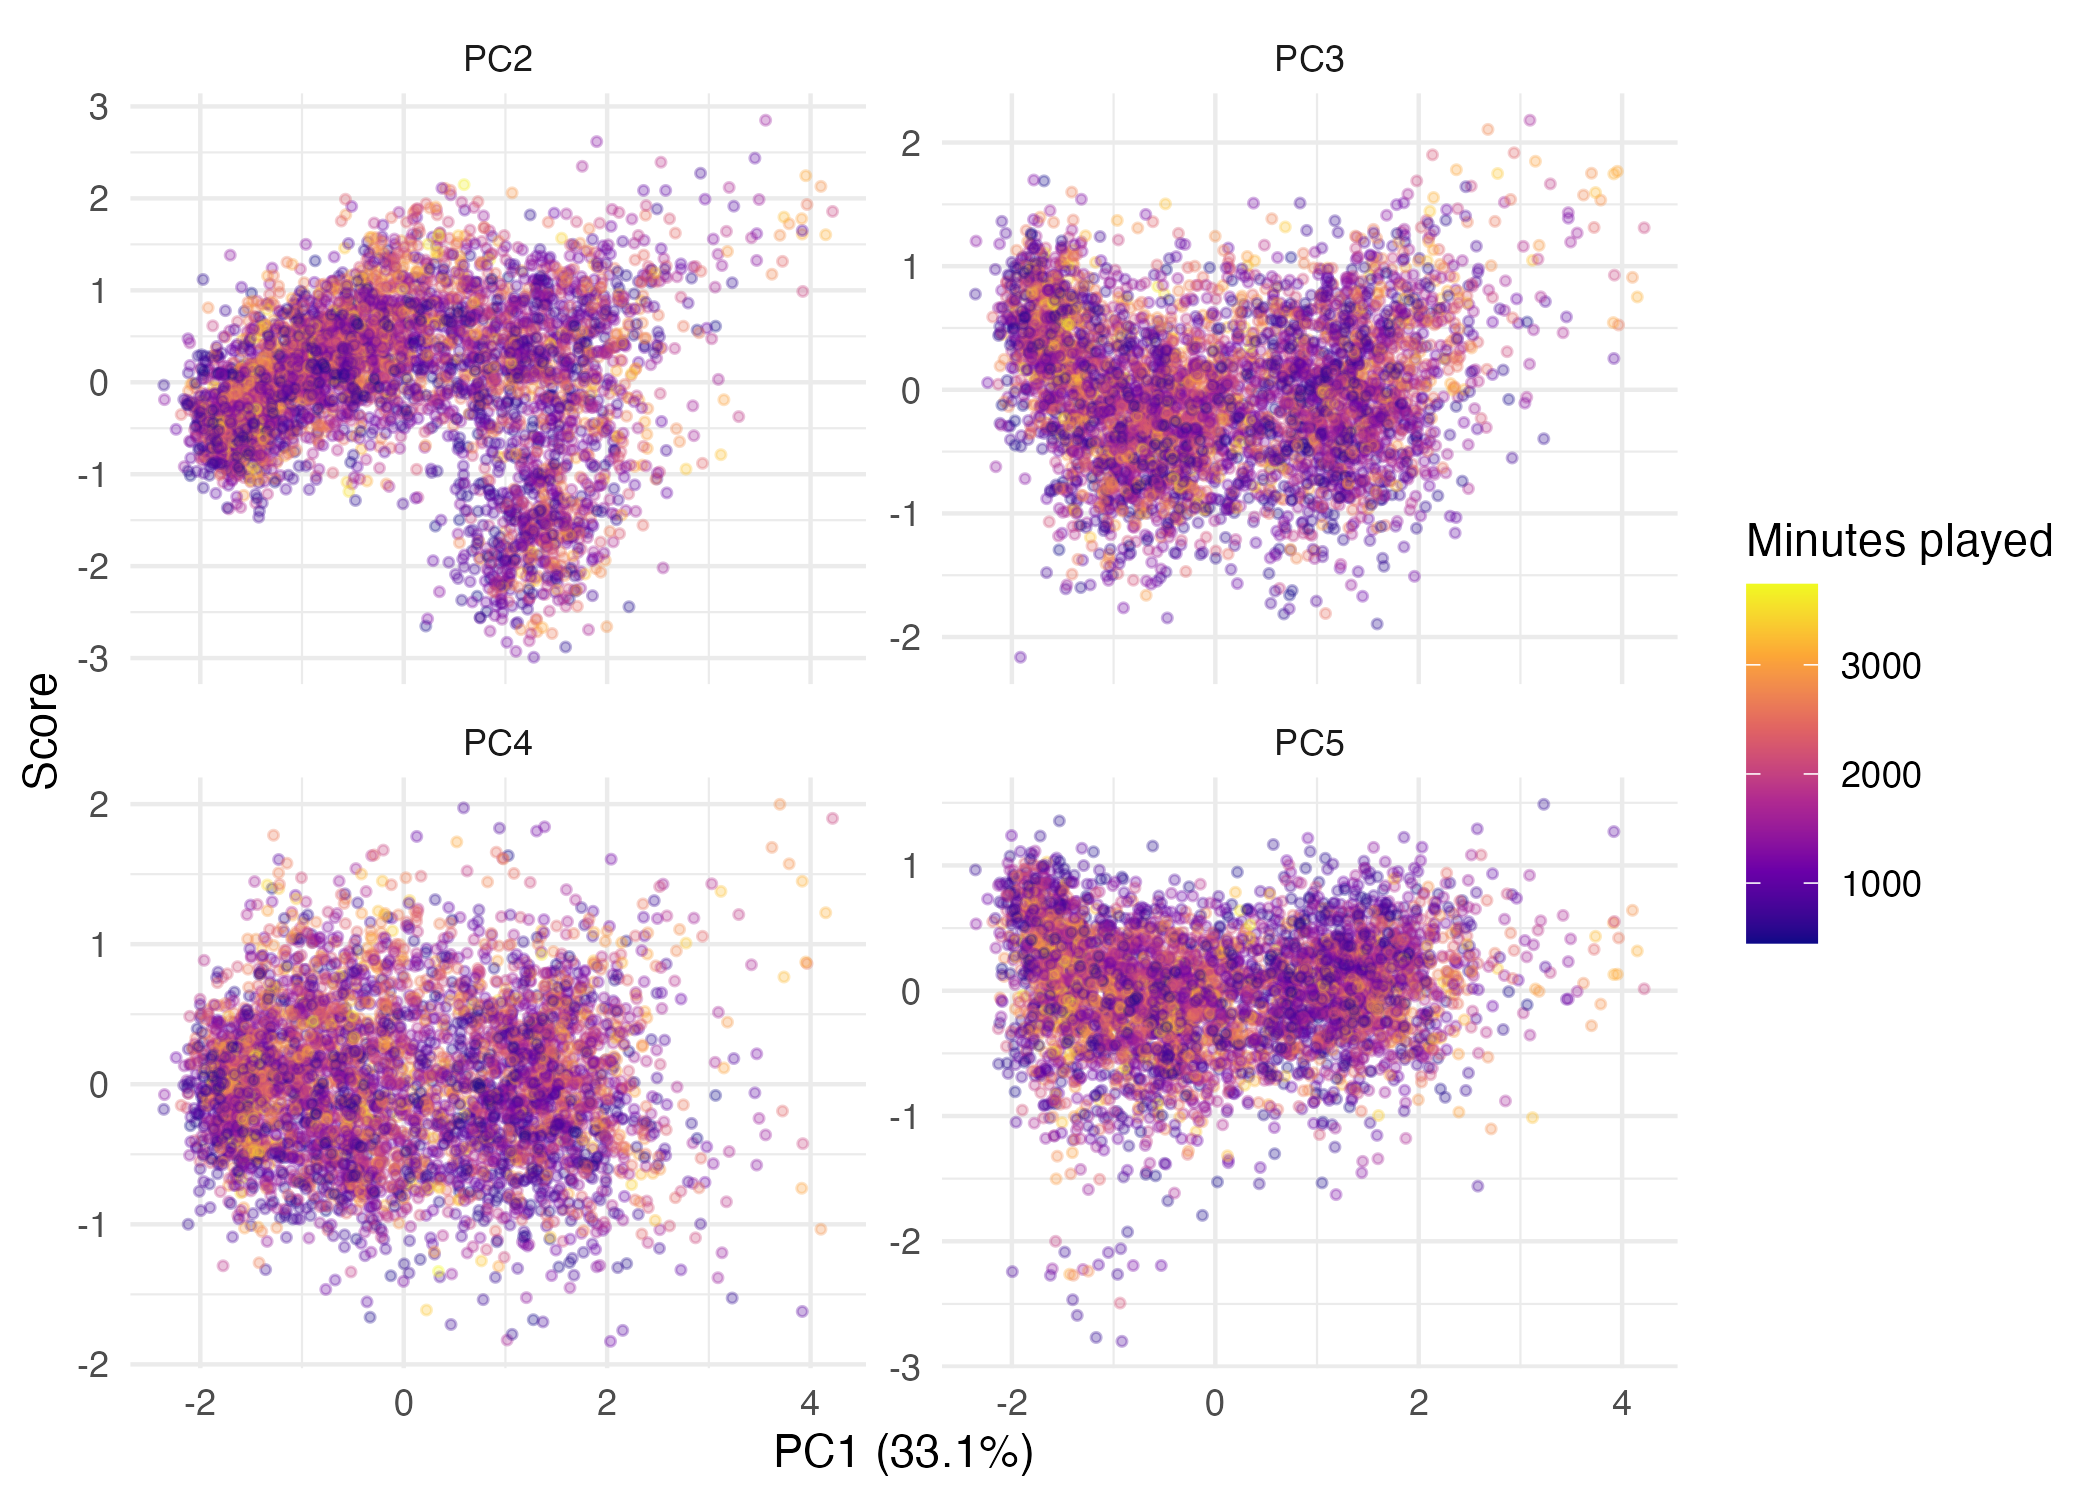
\includegraphics[width=0.8\textwidth]{images/scatter_pca.png}
    \caption{Principal component score plots for PC1 against PC2--PC5, with points coloured by minutes played. Playing time does not show a clear monotone gradient along the displayed components, suggesting that minutes played are not the main source of variation in the leading PCA scores.}
    \label{fig:pca_faceted_minutes}
\end{figure}

Although PCA is informative, its limitations are important. Each component is constructed to be uncorrelated with the previous ones because PCA imposes orthogonality on the extracted directions. This is a mathematical constraint of the method, not evidence that the underlying football traits are independent. For example, ball progression, chance creation, and attacking involvement may be substantively related even if their PCA summaries are forced to lie on orthogonal axes. PCA is therefore interpreted here as a descriptive compression of the transformed feature space, not as a structural model of latent football style.

\subsection{Factor analysis}

Factor analysis provides an alternative route to low-dimensional structure when the observed variables are thought to reflect a smaller number of underlying latent traits. In contrast to PCA, which is defined through variance-maximising linear projections, factor analysis begins from an explicit statistical model for the covariance structure of the observed variables \cite{bartholomew2011latent}.

\begin{definition}
A factor analysis model for observation \(i\), represented by a random vector \(\mathbf{Y}_i\in\mathbb{R}^p\), with \(k\) latent factors is given by
\[
\mathbf{Y}_i=\boldsymbol{\mu}+\mathbf{\Lambda}\mathbf{f}_i+\boldsymbol{\varepsilon}_i,
\]
where \(\boldsymbol{\mu}\in\mathbb{R}^p\) is a mean vector, \(\mathbf{f}_i\in\mathbb{R}^k\) is the latent factor vector for observation \(i\), \(\mathbf{\Lambda}\in\mathbb{R}^{p\times k}\) is a loading matrix, and \(\boldsymbol{\varepsilon}_i\in\mathbb{R}^p\) is an observation-specific residual vector. The matrix $\mathbf{\Lambda}$ describes how the observed variables depend linearly on the latent factors, while $\boldsymbol{\varepsilon}$ captures variable-specific residual variation not explained by the common factor structure \cite{bartholomew2011latent}.
\end{definition}

Under standard assumptions
\[
\mathbb{E}[\mathbf{f}_i]=\mathbf{0}, \qquad
\mathrm{Cov}(\mathbf{f}_i)=\mathbf{I}_k, \qquad
\mathbb{E}[\boldsymbol{\varepsilon}_i]=\mathbf{0}, \qquad
\mathrm{Cov}(\boldsymbol{\varepsilon}_i)=\mathbf{\Psi},
\]
where \(\mathbf{\Psi}=\mathrm{diag}(\psi_1,\ldots,\psi_p)\), and \(\mathbf{f}_i\) is independent of \(\boldsymbol{\varepsilon}_i\), it follows that
\[
\mathrm{Cov}(\mathbf{Y})=\mathbf{\Lambda}\mathbf{\Lambda}^\top+\mathbf{\Psi}.
\]
Thus, the covariance matrix is decomposed into a low-rank component, $\mathbf{\Lambda}\mathbf{\Lambda}^\top$, representing shared dependence among the variables, and a diagonal component, $\mathbf{\Psi}$, representing variable-specific residual variance.

This framework is appealing in football because the observed features are unlikely to be driven by wholly separate mechanisms. Variables related to progression and creation may share common structure, as may defensive activity and duel intensity, while finishing output may combine contributions from shot volume, box presence, and shot quality. In such a setting, a model that explains dependence through a smaller number of related latent traits is often more plausible than one based only on orthogonal descriptive directions.

Unlike PCA and CMDS, factor analysis is already a probabilistic model. For this thesis, factor analysis provides a simple latent-variable baseline for assessing whether the covariance structure of the player--season feature matrix can be represented through a number of interpretable latent dimensions before specifying a final Bayesian model.

In the exploratory analysis conducted here, after removing a constant feature with zero sample standard deviation, maximum-likelihood exploratory factor analysis was fitted for several candidate numbers of factors, followed by oblique rotation using an oblimin-type criterion in order to allow correlated factors \cite{bartholomew2011latent,jennrich1966rotation}.

The number of factors was guided in part by parallel analysis \cite{horn1965parallel}. Parallel analysis compares the observed eigenvalues of the empirical correlation matrix with eigenvalues obtained from random datasets of the same size. Factors are retained while the observed eigenvalues exceed a chosen simulated reference, here the simulated \(95\)th percentile. As shown in \autoref{fig:parallel_analysis}, the observed eigenvalues dominate the simulated reference eigenvalues up to the eleventh factor, after which the empirical curve falls below the simulated $95$th percentile. This provides empirical support for retaining eleven factors as a reasonable working dimension for the latent covariance structure; the larger count relative to a coarser feature set is expected, since \(P=48\) engineered features resolve considerably more distinct football sub-skills (e.g.\ separate passing-distance, duel-type, and defensive-action categories) than a smaller feature set would. Competing specifications were then compared using standard fit diagnostics.

More specifically, the root mean square residual (RMSR) summarises the average size of the residual correlations left unexplained by the fitted factor model, while the root mean square error of approximation (RMSEA) measures lack of fit per degree of freedom at the covariance-structure level \cite{bartholomew2011latent,browne1992fit}. Model comparison also considered the Bayesian information criterion (BIC), defined in the sense of Schwarz \cite{schwarz1978bic}, which balances model fit against complexity.

\begin{figure}[h]
    \centering
    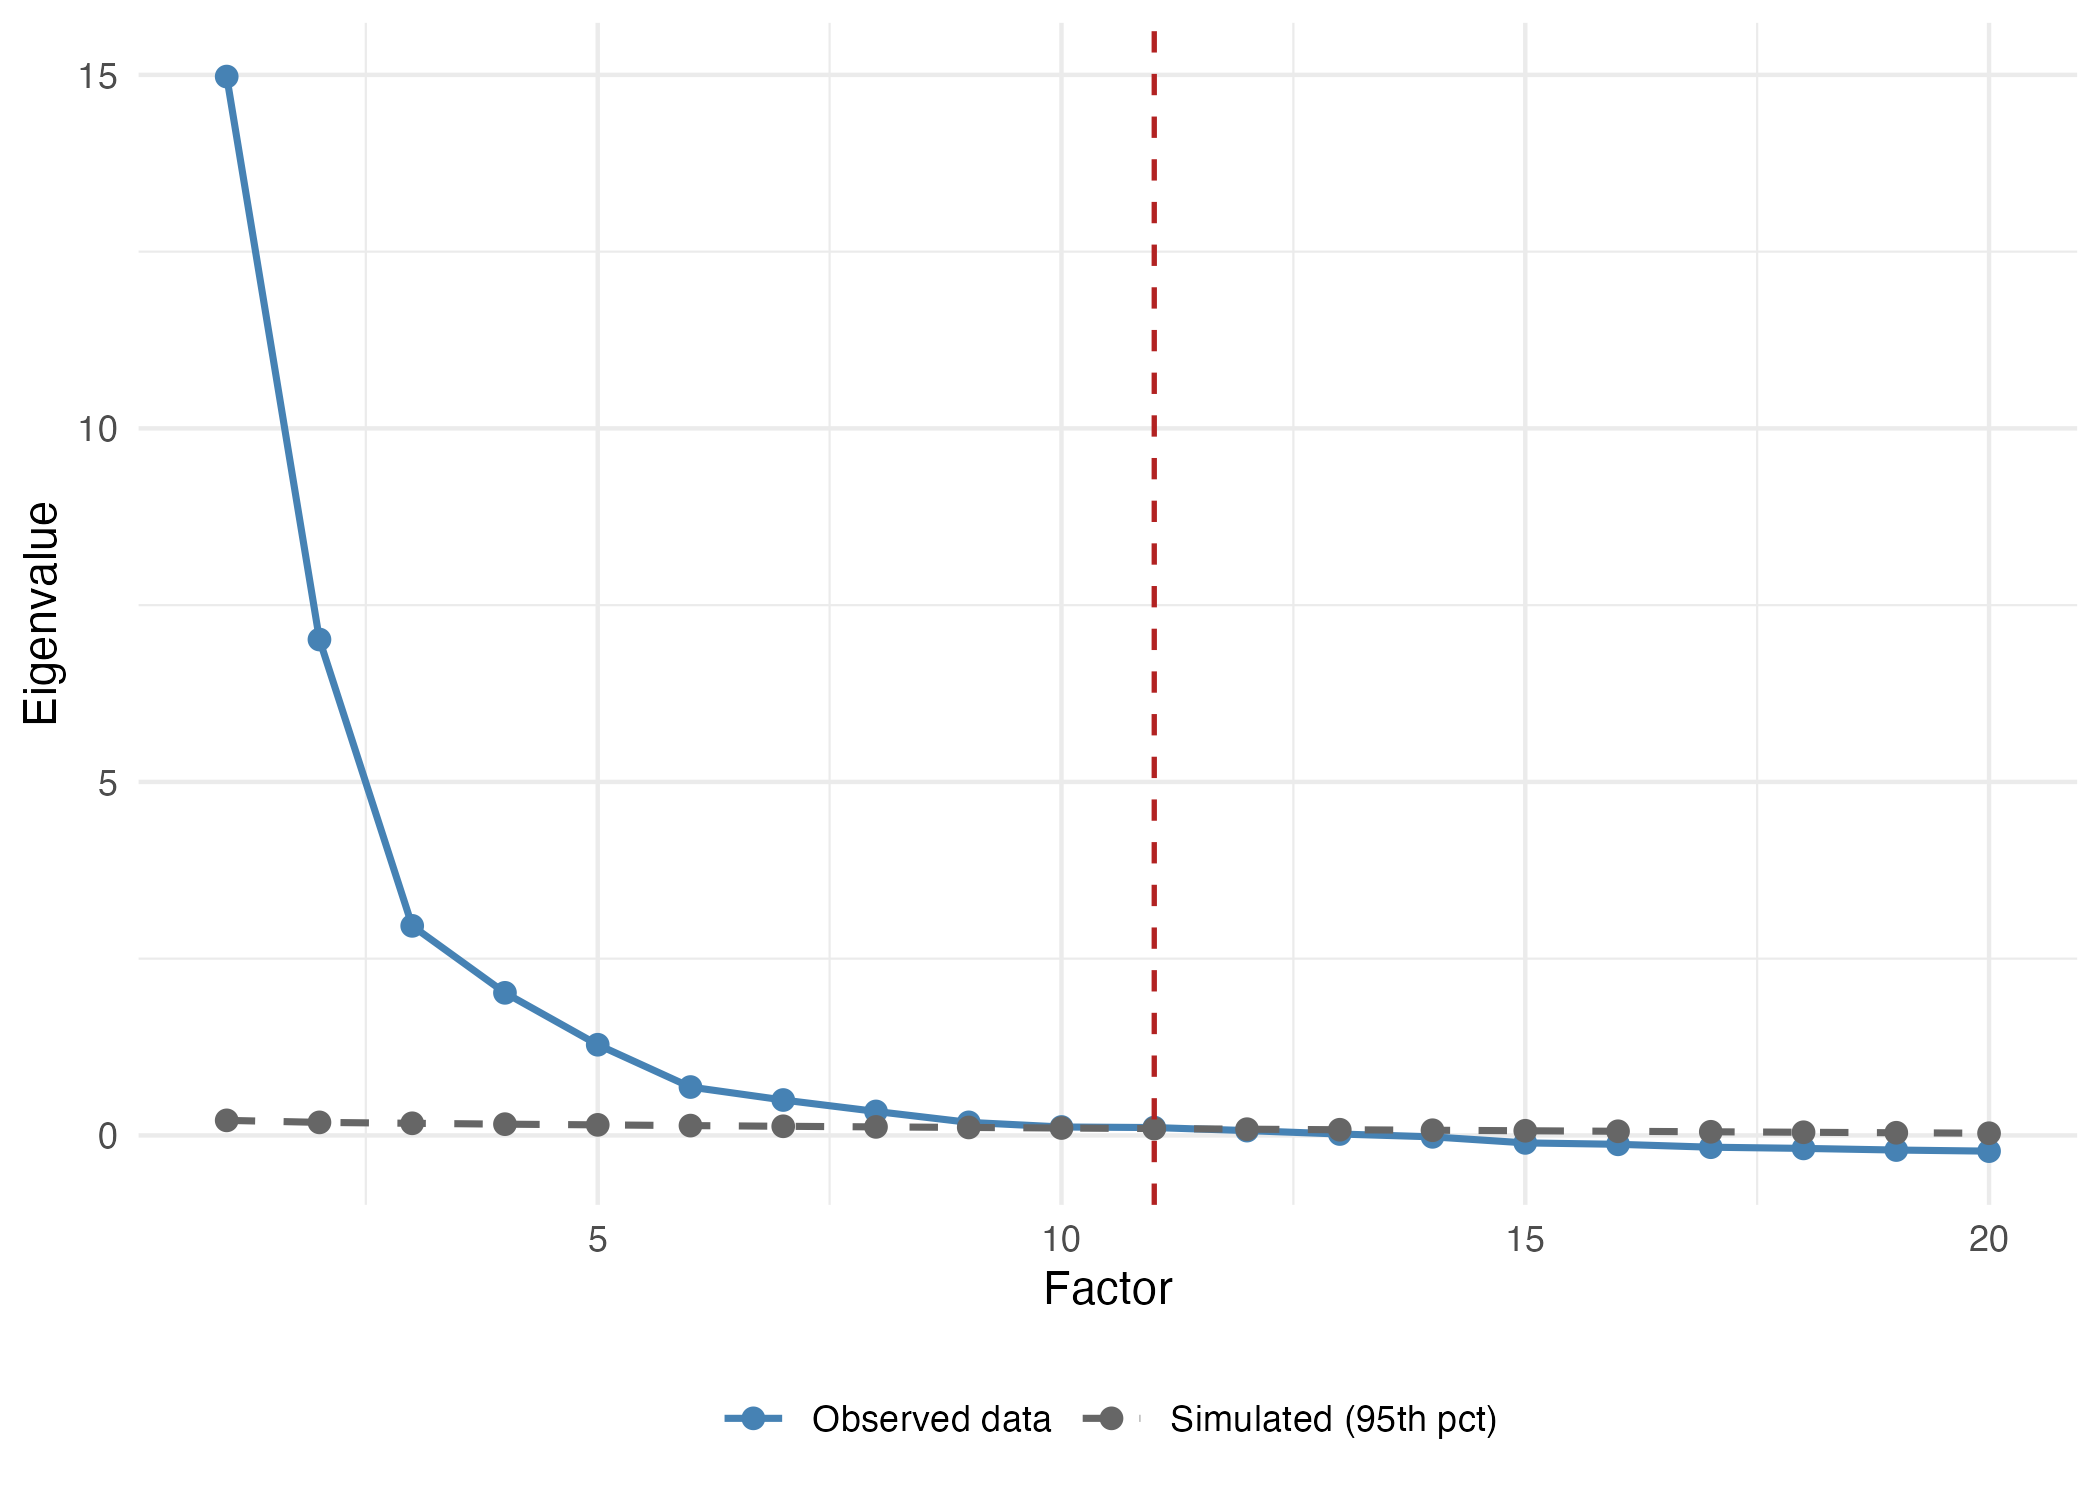
\includegraphics[width=0.8\textwidth]{images/scree_fa.png}
    \caption{Parallel analysis scree plot for factor analysis. The observed eigenvalues are compared with the $95$th percentile of eigenvalues obtained from simulated random datasets. The vertical dashed line indicates the suggested number of retained factors, $k=11$, corresponding to the point after which the observed eigenvalues no longer exceed the simulated reference values.}
    \label{fig:parallel_analysis}
\end{figure}

The exploratory results support the presence of non-trivial latent structure. Parallel analysis suggested an eleven-factor solution, while a nine-factor model provided a more compressed but rougher summary. The eleven-factor specification improved the fit statistics relative to the nine-factor one (TLI rising from \(0.804\) to \(0.843\); RMSEA falling from \(0.101\) to \(0.090\); RMSR falling from \(0.0256\) to \(0.0227\); BIC falling from approximately \(28{,}630\) to \(19{,}420\)), although the overall fit still indicates that the latent structure should be viewed as an approximation rather than a complete explanation of the dependence in the data. Taken together, the pattern in \autoref{fig:parallel_analysis} and the fit comparisons suggest that eleven factors offer a reasonable compromise between parsimony and interpretability for this larger, \(P=48\) feature set.

Substantively, the rotated loading structure reveals several interpretable latent dimensions; see \autoref{fig:fa_loadings}. Ordered by the variance each factor accounts for, the eleven-factor solution separates: chance creation and assists; goal threat and finishing; carrying and offensive duelling; general passing volume and circulation; defensive duel-winning and ball recovery; defensive duel exposure (1v1 defending workload); progressive and vertical passing; physical engagement and possession risk; high/pressing recoveries; passing accuracy versus crossing risk; and deep build-up circulation. While these labels are necessarily interpretive, the loading pattern shows that the latent dimensions are not arbitrary mathematical artefacts, but correspond to recognisable football behaviours -- including a clear separation, absent from a coarser feature set, between winning defensive duels and simply being exposed to them, and between general passing volume and specifically progressive, forward-directed passing. Importantly, the estimated factor correlations are not negligible (the strongest, between the chance-creation and carrying/offensive-duelling factors, reaches \(0.63\), and goal threat correlates negatively with both defensive factors at around \(-0.5\)), which reinforces the idea that football style may be better described through related latent traits than through a small set of orthogonal descriptive axes.

\begin{figure}[h]
    \centering
    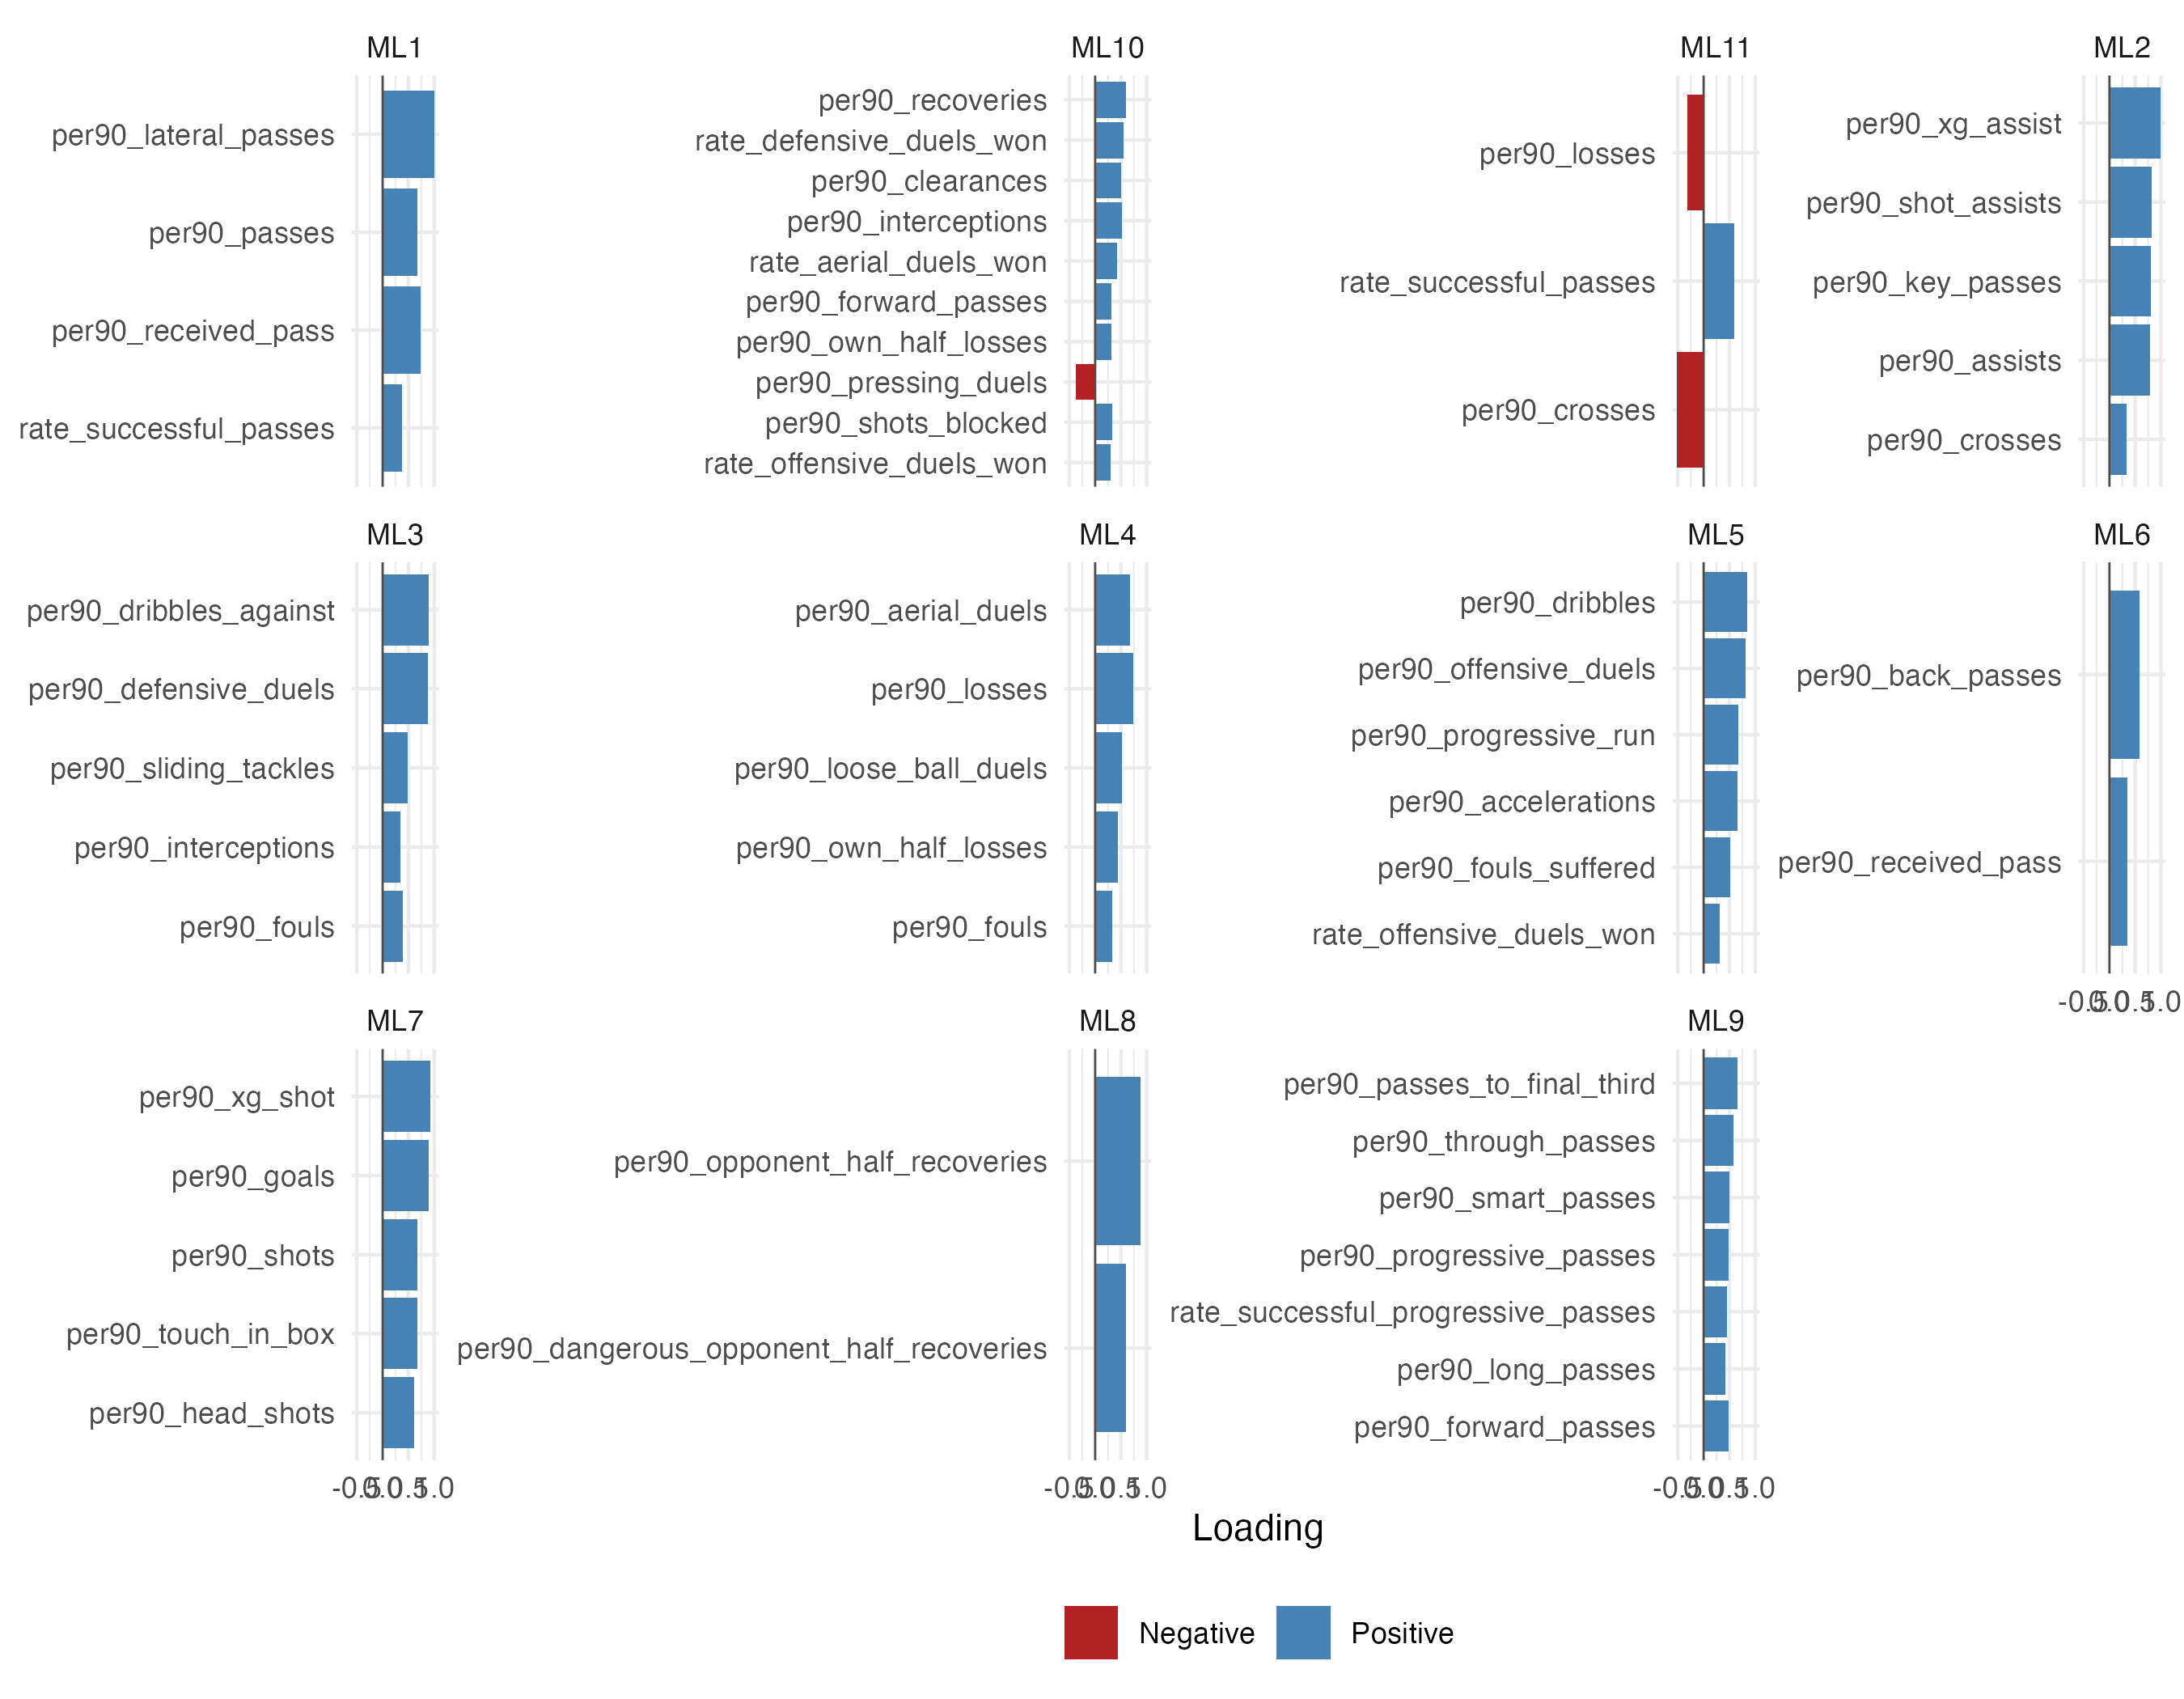
\includegraphics[width=0.8\textwidth]{images/loadings_fa.png}
    \caption{Rotated factor loadings for the eleven-factor oblimin solution, displaying variables with $|\mathrm{loading}|\geq 0.30$. Blue and red bars indicate positive and negative loadings, respectively. The loading pattern supports an interpretation of the factors in terms of chance creation, goal threat, carrying and offensive duelling, passing volume, defensive duel-winning, defensive duel exposure, progressive passing, physical engagement/possession risk, high-press recoveries, passing accuracy versus crossing, and deep build-up circulation.}
    \label{fig:fa_loadings}
\end{figure}

The role of factor analysis in this master's thesis is therefore both exploratory and strategic. It helps assess whether the transformed feature matrix supports an interpretable latent covariance structure, and it provides guidance for the construction of more refined probabilistic models later in the work. At the same time, it remains distinct from approaches based directly on pairwise dissimilarities, so its conclusions should be interpreted as one stage in a sequential modelling strategy rather than as the unique final representation of football similarity.

\subsection{Classical multidimensional scaling}

Classical multidimensional scaling (CMDS) starts from a matrix of pairwise dissimilarities rather than directly from the feature matrix. When those dissimilarities are ordinary Euclidean distances computed from centred feature vectors, CMDS is closely connected to PCA: the double-centred squared-distance matrix recovers the same principal-coordinate geometry as the PCA score representation. Its added value here is therefore not to duplicate PCA with Euclidean distances, but to examine non-Euclidean or profile-based dissimilarities, such as cosine-based dissimilarity. This makes it relevant here because one of the exploratory goals is to understand whether the similarity structure induced by the player--season representation can be expressed as a low-dimensional Euclidean configuration \cite{torgerson1958theory,borg2005mds,cox2001mds}.

Let $\mathbf{D}=(d_{ij})$ denote the matrix of pairwise dissimilarities between the $n$ observations, with $d_{ii}=0$, $d_{ij}=d_{ji}$, and let $q<n$ be a target embedding dimension. The CMDS problem is to construct points $\mathbf{z}_1,\ldots,\mathbf{z}_n\in\mathbb{R}^q$ such that the Euclidean interpoint distances $\|\mathbf{z}_i-\mathbf{z}_j\|$ approximate the observed dissimilarities as closely as possible. In its classical form, this is achieved through a spectral decomposition of a double-centred matrix of squared dissimilarities \cite{torgerson1958theory,borg2005mds}.

\begin{theorem}
Suppose that $\mathbf{D}^{(2)}=(d_{ij}^2)$ is the matrix of squared pairwise Euclidean distances generated by some centred configuration of $n$ points in $\mathbb{R}^m$. Let
\[
\mathbf{J}=\mathbf{I}_n-\frac{1}{n}\mathbf{1}\mathbf{1}^\top
\]
be the centring matrix, and define
\[
\mathbf{B}=-\frac{1}{2}\mathbf{J}\mathbf{D}^{(2)}\mathbf{J}.
\]
Then $\mathbf{B}$ is the Gram matrix of the centred configuration. If
\[
\mathbf{B}=\mathbf{V}\mathbf{\Lambda}\mathbf{V}^\top
\]
is its spectral decomposition, then the coordinates of the configuration can be recovered, up to rigid transformations, as
\[
\mathbf{Z}=\mathbf{V}\mathbf{\Lambda}^{1/2}.
\]
If only the first $q$ positive eigenvalues are retained, so that
\[
\mathbf{Z}_q=\mathbf{V}_q\mathbf{\Lambda}_q^{1/2},
\]
then $\mathbf{Z}_q$ provides the best rank-$q$ approximation to $\mathbf{B}$ in the least-squares sense given by the Eckart--Young theorem, and hence the classical $q$-dimensional CMDS representation obtained through spectral truncation \cite{torgerson1958theory,cox2001mds,borg2005mds}.
\end{theorem}

Thus, the double-centred matrix provides a closed-form route to principal coordinates when the input dissimilarities are squared Euclidean distances. In that case, CMDS is essentially a distance-based route to the same geometry obtained from PCA on the centred data. When the input dissimilarities are not squared Euclidean, as with cosine-based dissimilarity in the present exploratory analysis, the same spectral procedure gives an approximate Euclidean representation of that dissimilarity structure \cite{cox2001mds,borg2005mds}. In practice, the eigenvalue pattern of $\mathbf{B}$ is therefore informative about whether the distance structure is close to low-dimensional Euclidean and about how much information is lost when only a few dimensions are retained.

In the present work, CMDS was applied in particular to the cosine-based dissimilarity matrix. This matrix should be understood as an angular-based dissimilarity matrix rather than as a strict metric distance matrix. Cosine-based dissimilarity emphasizes the direction of the player profile rather than its overall norm, and when vectors are centred this directional comparison is equivalent to correlation. In this sense, two player--season observations may be regarded as similar not because they have the same absolute output, but because they exhibit a similar pattern across features. For example, two players with very different total event volumes may still be close under cosine-based dissimilarity if both display the same relative emphasis on progression, dribbling, defensive work, and duel involvement. CMDS then provides a first low-dimensional map of this pattern-based similarity structure.

\begin{figure}[h]
    \centering
    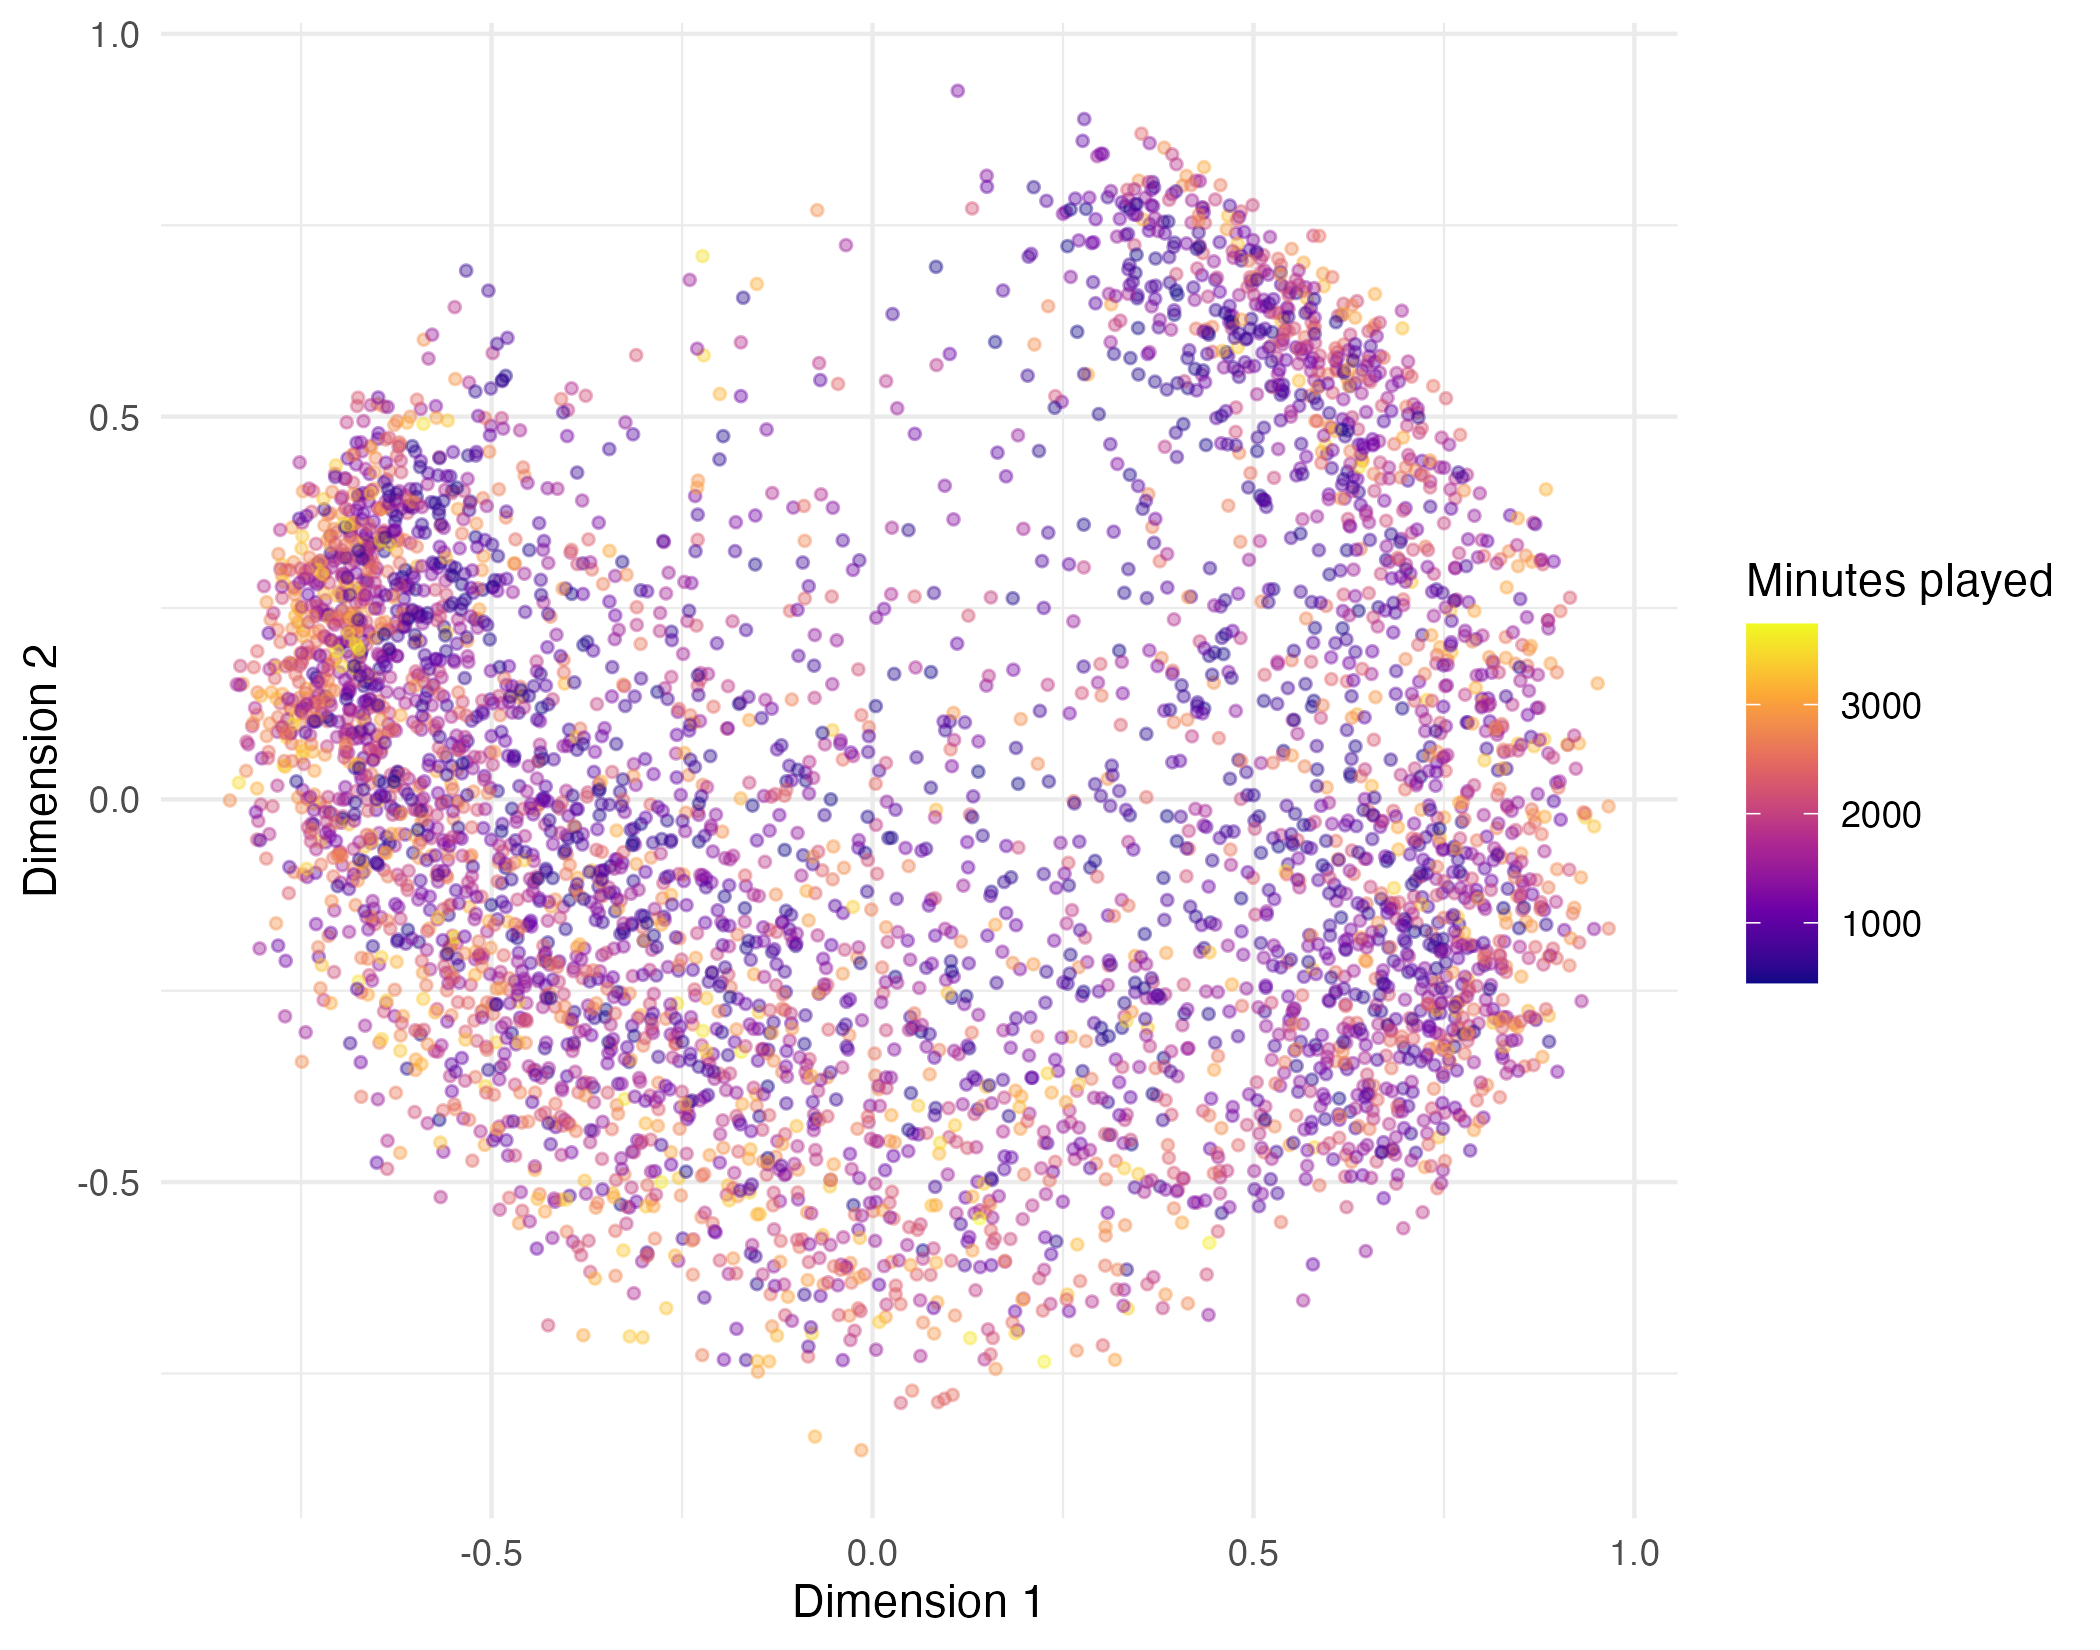
\includegraphics[width=0.8\textwidth]{images/cmds_cosine.png}
    \caption{Two-dimensional CMDS embedding of the player--season observations using cosine-based dissimilarity. Points are coloured by minutes played. The absence of a clear minutes gradient suggests that the embedding is not primarily driven by playing time.}
    \label{fig:cmds_cosine}
\end{figure}

This representation is useful for exploratory purposes. It allows one to inspect whether the player--season observations occupy a coherent geometric space, whether certain profiles appear as extremes of the representation, and whether metadata-defined subsets of the data---for instance observations from different seasons, positional groups, or usage levels---occupy comparable regions of the map. At the same time, the limitations of CMDS are clear. It yields a deterministic embedding rather than a probabilistic one, provides no direct quantification of uncertainty for player locations, and does not by itself account for repeated observations of the same player across seasons or for more structured hierarchical variation.

\begin{figure}[h]
    \centering
    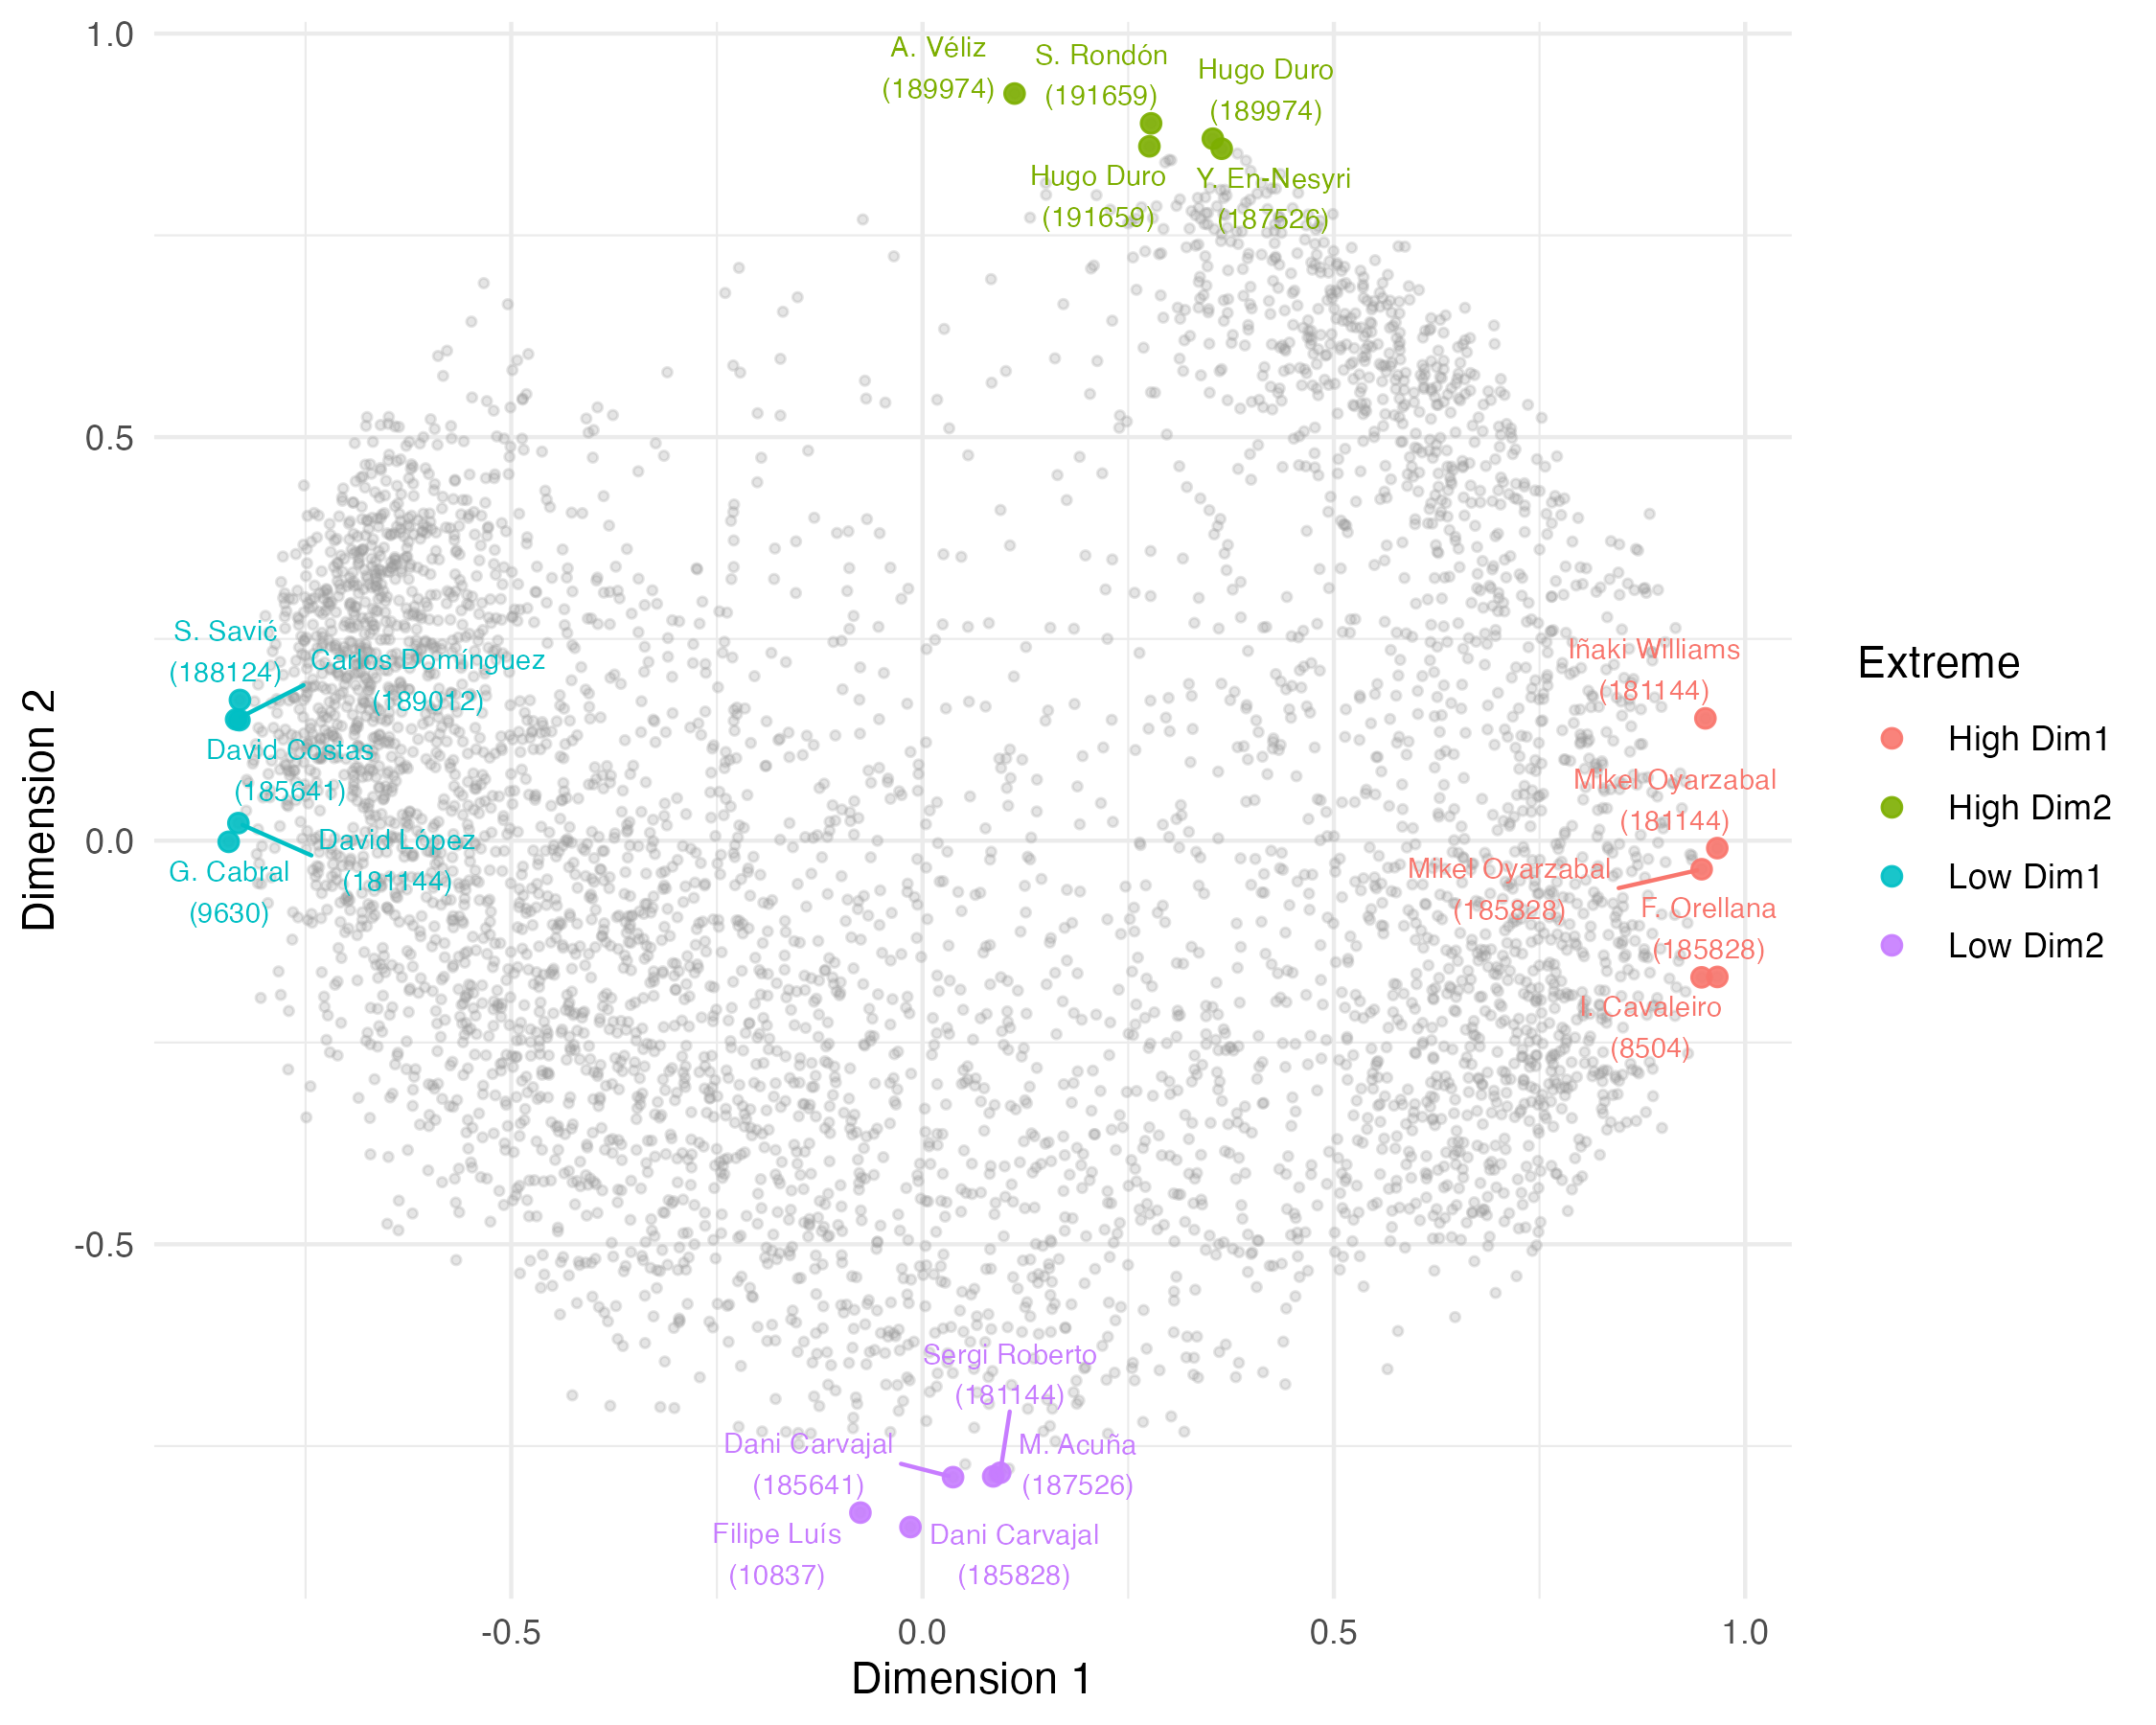
\includegraphics[width=0.8\textwidth]{images/cmds_extreme_obs.png}
    \caption{CMDS map with extreme observations labelled. The four groups of extremes correspond to high and low values along each displayed dimension. Dimension 1 is mainly anchored by wide attacking profiles on the positive side and centre-back profiles on the negative side, while Dimension 2 contrasts aerial or box-reference forwards with attacking full-back profiles.}
    \label{fig:cmds_extremes}
\end{figure}

The labelled extremes in \autoref{fig:cmds_extremes} help interpret the two displayed dimensions. The positive side of Dimension 1 is anchored mainly by wide attacking profiles, such as F. Orellana, Mikel Oyarzabal, Iñaki Williams, and I. Cavaleiro, whereas the negative side contains centre-back profiles, such as G. Cabral, Carlos Domínguez, David López, David Costas, and S. Savić. Dimension 2 separates aerial or penalty-box reference forwards, such as A. Véliz, S. Rondón, Hugo Duro, and Y. En-Nesyri, from attacking full-back profiles with substantial progression involvement, such as Dani Carvajal, Filipe Luís, M. Acuña, and Sergi Roberto. These labels should be interpreted descriptively: they identify the observed profiles anchoring the CMDS axes, not fixed universal football roles.  For these reasons, CMDS is best viewed here as an exploratory geometric benchmark rather than as the final model. It indicates whether the chosen dissimilarity admits a coherent low-dimensional approximation, and it provides a descriptive precursor to more structured probabilistic latent-space models, including Bayesian and hierarchical extensions \cite{oh2001bayesian,yanchenko2020hierarchical}.

\subsection{Summary of the exploratory role of PCA, FA, and CMDS}

Taken together, PCA, FA, and CMDS provide complementary descriptive evidence that the player--season data contain meaningful lower-dimensional structure. PCA suggests that a moderate number of directions captures a large proportion of total variation. FA indicates that several correlated latent traits may underlie the observed features. CMDS shows that the pairwise dissimilarity structure admits an interpretable low-dimensional Euclidean approximation.

These findings do not by themselves determine the final model, but they justify moving towards a latent-space formulation. More importantly, they reveal that the data contain enough structure for such a model to be meaningful, while also making clear that a purely descriptive approach is insufficient if one wishes to quantify uncertainty and account for the longitudinal character of player--season observations.